\chapter{Motivation}\label{ch:motivation}

The rapid evolution of cellular users in recent years, refer to \cref{fig:cellular_subscriptions}, has significantly increased the demand for high-speed, reliable data connectivity. This growing demand has placed substantial pressure on existing network infrastructures, requiring new solutions to enhance both capacity and coverage.\ \glspl{hetnet} have been proposed as an effective strategy to address these challenges by creating multi-layered networks that enable efficient data offloading \autocite{xu2021survey}. This improves both the capacity and coverage across the network. However, the dense deployment of these networks also increases energy consumption, which is undesirable in today's environmentally conscious and cost-sensitive world.

\begin{figure}
  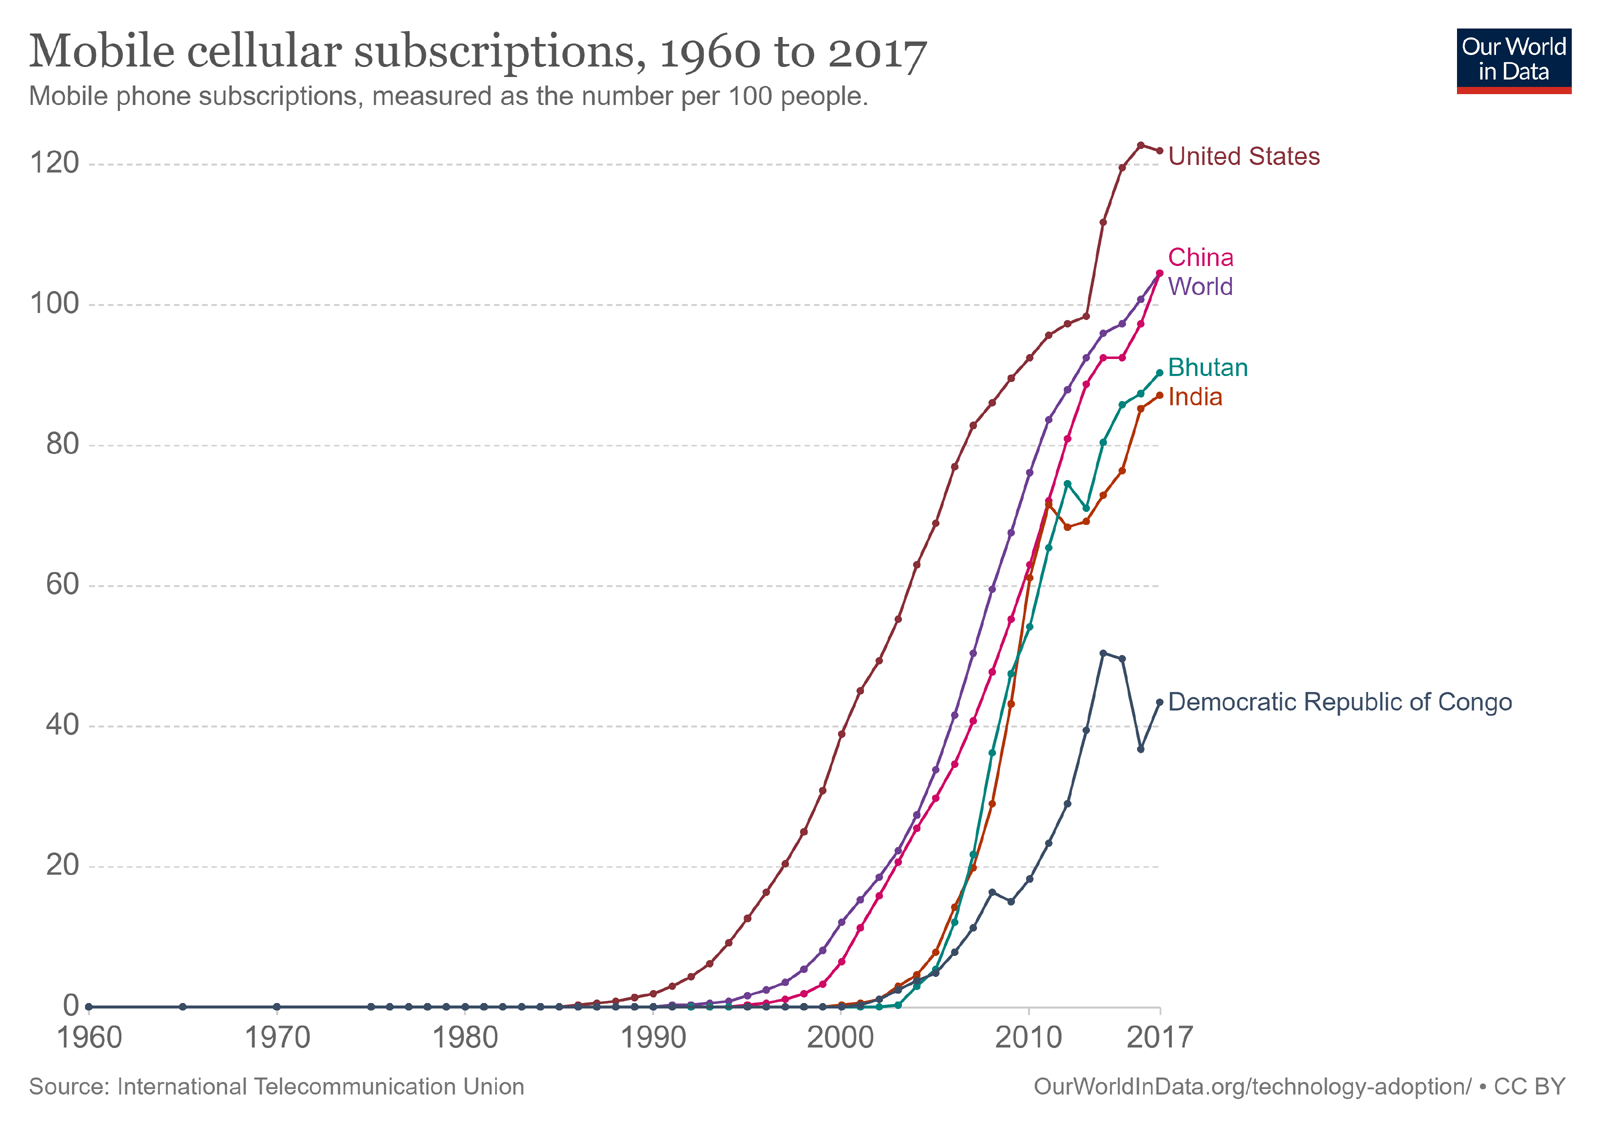
\includegraphics{mobil_cellular_subscriptions_graph.png}
  \caption{Global Trends in Mobile Cellular Subscriptions (1960–2017): The graph illustrates the exponential growth of mobile subscriptions per 100 people across various regions over recent decades. \autocite{pahoInformationSystems}}\label{fig:cellular_subscriptions}
\end{figure}

Reducing power consumption while maintaining \gls{qos} requirements has therefore become a key objective in the deployment and operation of mobile networks \autocite{lopezperez2022survey}. In this context, \glspl{ntn} have emerged as a promising approach to complement \glspl{tn} and expand coverage to regions that have historically been underserved due to the prohibitive costs or logistical challenges of deploying terrestrial base stations \autocite{ahmmed2022digital}.

\glspl{ntn} leverage airborne platforms, including \gls{uav}, \glspl{hap}, and satellites, to act as relay nodes or base stations, providing connectivity to end-users across vast geographical areas. Their key advantage lies in the ability to cover expansive regions, including remote and inaccessible areas, where terrestrial solutions are either too costly or impractical. In particular, \gls{leo} satellites, which orbit at altitudes between 200 and 2000 kilometers, have shown significant potential for providing high-capacity connectivity due to their lower latency and stronger signal strength compared to other satellite types \autocite{giordani2021non}. This proximity to Earth not only enhances performance but also reduces energy requirements, aligning with the broader goal of minimizing power consumption in modern networks.

The emergence of \glspl{ntn} has further enabled the development of advanced concepts such as the \gls{istn} \autocite{ao2018space}\autocite{huang2019airplane}\autocite{liu2022operation}, and the \gls{iost} \autocite{akyildiz2019internet}\autocite{priyadarshini2022novel}\autocite{kak2021designing}. These concepts envision a seamless integration of terrestrial and non-terrestrial components to deliver next-generation communication services, particularly for future \gls{6g} networks. Mega-constellations of satellites, exemplified by networks like Starlink \autocite{tao2022impact} and OneWeb \autocite{zhu2022laser}, are at the forefront of this transformation. By integrating these networks with terrestrial systems, it becomes possible to connect isolated regions, including rural and oceanic environments, which are otherwise challenging to serve. Furthermore, this integration holds the potential to create a unified communication infrastructure that offers connectivity not only on the ground but also in the air and space.

This research is motivated by the growing need to develop sustainable, cost-effective solutions for extending connectivity to remote areas. \glspl{ntn}, particularly when integrated with \glspl{tn}, present a viable path forward in addressing these challenges, thereby supporting the goals of global connectivity and reducing energy consumption in future wireless communication systems. The work is supported by ongoing efforts in \glspl{ntn} to leverage emerging technologies for the development of \gls{6g} networks, with the ultimate aim of delivering ubiquitous, high-quality communication services to all corners of the world.

% Local Variables:
% jinx-local-words: "hetnet ntn qos uav"
% End:
